\usepackage{ifthen}

% Define an agenda item
%
% Arguments:
% 1: Identifier of the agenda item, should be all lower-case
% 2: Type of the agenda item: lecture or lab
% 3: English title of the agenda item
% 4: English full description of the agenda item
% 5: French title of the agenda item
% 6: French full description of the agenda item
\newcommand\defagendaitem[6]{
  \ifthenelse{\equal{\agendalanguage}{french}}{
    \expandafter\def\csname #1@#2@title\endcsname {#5}
    \expandafter\def\csname #1@#2@contents\endcsname {#6}
  }{
    \expandafter\def\csname #1@#2@title\endcsname {#3}
    \expandafter\def\csname #1@#2@contents\endcsname {#4}
  }
}

% Show/render an agenda item
%
% Arguments:
% 1: Identifier of the agenda item, as defined by \defagendaitem
% 2: Type of the agenda item: lecture or lab
\newcommand\showagendaitem[2]{%
  \ifthenelse{\boolean{hlineneeded}}{\\\hline}{\setboolean{hlineneeded}{true}}%
    \ifthenelse{\equal{\agendalanguage}{french}}{%
      \ifthenelse{\equal{#2}{lecture}}%
      {Cours &}%
      {%
        \ifthenelse{\equal{#2}{lab}}{%
          \ifthenelse{\equal{\trainingtype}{online}}{Démo &}{TP &}%
        }%
        {}%
      }%
    }{%
      \ifthenelse{\equal{#2}{lecture}}%
      {Lecture &}%
      {%
        \ifthenelse{\equal{#2}{lab}}{%
          \ifthenelse{\equal{\trainingtype}{online}}{Demo &}{Lab &}%
        }%
        {}%
      }%
    }%
    \csname #1@#2@title\endcsname &%
    \vspace{-12pt}%
    \csname #1@#2@contents\endcsname%
}%

% Define a board
%
% Arguments:
% 1: Identifier for the board, must be all lower-case
% 2: English title
% 3: English full description
% 4: French title
% 5: French full description
% 6: Board picture
\newcommand\defboard[6]{
  \ifthenelse{\equal{\agendalanguage}{french}}{
    \expandafter\def\csname #1@title\endcsname {#4}
    \expandafter\def\csname #1@contents\endcsname {#5}
  }{
    \expandafter\def\csname #1@title\endcsname {#2}
    \expandafter\def\csname #1@contents\endcsname {#3}
  }
  \expandafter\def\csname #1@image\endcsname {#6}
}

% Show/render a board
%
% Arguments:
% 1: Identifier of the board, as defined by \defboard
\newcommand\showboarditem[1]{
  \begin{tabularx}{\textwidth}{p{7cm}p{11cm}}
    \arrayrulecolor{blorange}
    \hline
    \multicolumn{1}{l}{\textbf{\textcolor{blorange}{\large \csname #1@title\endcsname}}} & \\
    \hline
    \arrayrulecolor{gray}
    \csname #1@contents\endcsname &
    \csname #1@image\endcsname \\
  \end{tabularx}
}

% Start an agenda by finding
% out if it is a morning or an
% afternoon if the training
% takes place on site
%
% Arguments:
% 1: Number of the half-day
\newcommand\showagendaday[1]{%
  \arrayrulecolor{blorange}%
  \\\hline%
  \multicolumn{3}{l}{%
    \textbf{\textcolor{blorange}{\large%
      \ifthenelse{\equal{\trainingtype}{online}}{%
        \showonlineagendaday{#1}%
      }{%
        \pgfmathparse{int(mod(#1, 2))}%
        \ifnum\pgfmathresult=1%
          \pgfmathparse{int((#1 + 1) / 2)}%
          \showonsiteagendaday{\pgfmathresult}{morning}%
        \else%
          \pgfmathparse{int(#1 / 2)}%
          \showonsiteagendaday{\pgfmathresult}{afternoon}%
        \fi%
      }%
    }}%
  } \\%
  \hline%
  \setboolean{hlineneeded}{false}%
  \arrayrulecolor{gray}%
}%

% Start an online agenda half-day
%
% Arguments:
% 1: Number of the half-day
\newcommand\showonlineagendaday[1]{%
  \ifthenelse{\equal{\agendalanguage}{french}}{%
    Demi-journée #1%
  }{%
    Half day #1%
  }%
}%

% Start an on-site agenda half-day
%
% Arguments:
% 1: Number of the day
% 2: "morning" or "afternoon"
\newcommand\showonsiteagendaday[2]{%
  \ifthenelse{\equal{\agendalanguage}{french}}{%
    \ifthenelse{\equal{#2}{morning}}{%
      Jour #1 - Matin%
    }{%
      Jour #1 - Après-midi%
    }%
  }{%
    \ifthenelse{\equal{#2}{morning}}{%
      Day #1 - Morning%
    }{%
      Day #1 - Afternoon%
    }%
  }%
}%

\defboard
{stm32mp1}
{STM32MP1 Discovery Kit}
{
  One of these Discovery Kits from STMicroelectronics: {\bf
  STM32MP157A-DK1}, {\bf STM32MP157D-DK1}, {\bf STM32MP157C-DK2} or
  {\bf STM32MP157F-DK2}
  \begin{itemize}
  \item STM32MP157, dual Cortex-A7 processor from STMicroelectronics
  \item USB powered
  \item 512 MB DDR3L RAM
  \item Gigabit Ethernet port
  \item 4 USB 2.0 host ports
  \item 1 USB-C OTG port
  \item 1 Micro SD slot
  \item On-board ST-LINK/V2-1 debugger
  \item Arduino compatible headers
  \item Audio codec, buttons, LEDs
  \item LCD touchscreen (DK2 kits only)
  \vspace{-0.7cm}
  \end{itemize}
}
{Plateforme STM32MP1}
{
  Une de ces cartes de STMicroelectronics : {\bf
  STM32MP157A-DK1}, {\bf STM32MP157D-DK1}, {\bf STM32MP157C-DK2} ou
  {\bf STM32MP157F-DK2}
  \begin{itemize}
  \item Processeur STM32MP157, double Cortex-A7, de STMicroelectronics
  \item Alimentée par USB
  \item 512 Mo DDR3L RAM
  \item Port Gigabit Ethernet port
  \item 4 ports hôte USB 2.0
  \item 1 port USB-C OTG
  \item 1 connecteur Micro SD
  \item Debugger ST-LINK/V2-1 sur la carte
  \item Connecteurs compatibles Arduino Uno v3
  \item Codec audio
  \item Divers : boutons, LEDs
  \item Écran LCD tactile (uniquement sur cartes DK2)
  \vspace{-0.7cm}
  \end{itemize}
}
{
  \begin{center}
    \includegraphics[width=5cm]{../slides/discovery-board-dk1/discovery-board-dk1.png}
  \end{center}
}

\defagendaitem
{qna}
{misc}
{Questions and Answers}
{
  \begin{itemize}
  \item Questions and answers with the audience about the course topics
  \item Extra presentations if time is left, according what most
        participants are interested in.
  \end{itemize}
}
{Questions / réponses}
{
  \begin{itemize}
  \item Questions et réponses avec les participants à propos des sujets abordés.
  \item Présentations supplémentaires s'il reste du temps, en fonction des demandes
        de la majorité des participants.
  \end{itemize}
}


\defboard
{beagleboneblack}
{BeagleBone Black}
{
  {\bf BeagleBone Black} or {\bf BeagleBone Black Wireless} board
  \begin{itemize}
  \item An ARM AM335x (single Cortex-A8) processor from Texas
    Instruments
  \item USB powered
  \item 512 MB of RAM
  \item 2 or 4 GB of on-board eMMC storage
  \item USB host and device
  \item HDMI output
  \item 2 x 46 pins headers, to access UARTs, SPI buses, I2C buses
    and more.
  \item Ethernet or WiFi
  \end{itemize}
  \vspace{-0.7cm}
}
{BeagleBone Black}
{
  Carte {\bf BeagleBone Black} ou {\bf BeagleBone Black Wireless}
  \begin{itemize}
  \item Un processeur ARM AM335x de Texas Instruments (à base de
    Cortex-A8), avec accélération 3D, etc.
  \item 512 Mo de RAM
  \item 2 ou 4 Go de stockage eMMC
  \item USB hôte et device
  \item Sortie HDMI
  \item Connecteurs à 2 x 46 broches, pour accéder aux UARTs, aux bus
    SPI, aux bus I2C, et à d'autres entrées/sorties du processeur.
  \item Ethernet ou WiFi
  \vspace{-0.7cm}
  \end{itemize}
}
{
  \begin{center}
    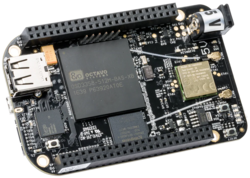
\includegraphics[width=5cm]{../slides/beagleboneblack-board/beagleboneblack_sd.png}
  \end{center}
}

\defboard
{beagleplay}
{BeaglePlay}
{
  {\bf BeaglePlay} board
  \begin{itemize}
    \item Texas Instruments AM625x (4xARM Cortex-A53 CPU)
    \item SoC with 3D acceleration, integrated MCU and many other peripherals.
    \item 2 GB of RAM
    \item 16 GB of on-board eMMC storage
    \item USB host and USB device, microSD, HDMI
    \item 2.4 and 5 GHz WiFi, Bluetooth and also Ethernet
    \item 1 MicroBus Header (SPI, I2C, UART, ...), OLDI and CSI connector.
  \vspace{-0.7cm}
  \end{itemize}
}
{BeaglePlay}
{
  Carte {\bf BeaglePlay}
  \begin{itemize}
    \item SoC Texas Instruments AM625x (CPU 4xARM Cortex-A53)
    \item SoC avec accélération 3D, MCU intégré et de nombreux autres périphériques.
    \item 2 GB de RAM
    \item 16 Go de stockage eMMC
    \item USB hôte et device, microSD, HDMI
    \item WiFi 2.4 and 5 GHz, Bluetooth et aussi Ethernet
    \item 1 Header MicroBus (SPI, I2C, UART, ...), connecteurs OLDI et CSI.
  \vspace{-0.7cm}
  \end{itemize}
}
{
  \begin{center}
    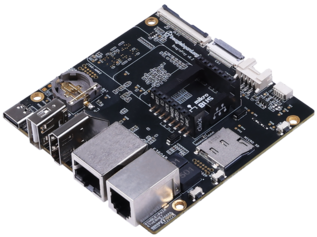
\includegraphics[width=5cm]{../slides/beagleplay-board/beagleplay_sd.png}
  \end{center}
}

\defboard
{espressobin}
{Hardware platform for practical labs}
{
  {\bf Globalscale EspressoBin} board
  \begin{itemize}
  \item Dual Cortex A53 Marvell Armada 3720 SoC
  \item Onboard switch with 2x 1Gbps interfaces
  \item Extra 1Gbps interface
  \item 1GB RAM
  \item 1x SATA interface
  \item 1x USB 3.0 interface
  \end{itemize}
}
{Plateforme matérielle pour les travaux pratiques}
{
  Carte {\bf Globalscale EspressoBin}
  \begin{itemize}
  \item SoC Marvell Armada 3720 SoC (CPU 2xARM Cortex A53)
  \item Switch Ethernet avec 2 interfaces Gigabit
  \item Interface Gigabit Ethernet additionnelle
  \item 1GB de RAM
  \item 1x interface SATA
  \item 1x interface USB 3.0
  \end{itemize}
}
{
  \begin{center}
    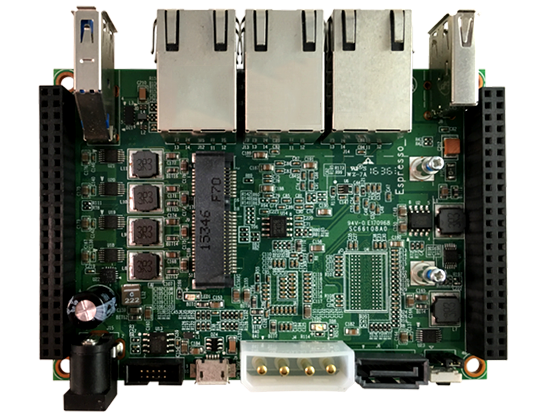
\includegraphics[width=5cm]{../slides/espressobin/espressobin.png}
  \end{center}
}


\def \training{graphics}

% Title
\ifthenelse{\equal{\agendalanguage}{french}}{
  \def \trainingtitle{Formation Comprendre la stack graphique sous Linux}
}{
  \def \trainingtitle{Understanding the Linux Graphics Stack training}
}

% Duration
\ifthenelse{\equal{\trainingtype}{online}}{
  \def \trainingduration{4}
}{
  \def \trainingduration{2}
}

% Training objectives
\ifthenelse{\equal{\agendalanguage}{french}}{
  \def \traininggoals{
    \begin{itemize}
    \item Être capable de comprendre les bases de l'affichage graphique: représentation
      des images et des couleurs, affichage de pixels, opérations sur
      les pixels.
    \item Être capable de comprendre le matériel lié à l'affichage graphique: composants
      du {\em pipeline} graphique, matériel pour le rendu et l'affichage
      graphique.
    \item Avoir une compréhension claire des composants de la pile
      logicielle pour le graphique dans le noyau Linux et de leurs
      rôles: TTY, sous-systèmes {\em framebuffer} et DRM.
    \item Avoir une compréhension claire de la pile logicielle pour le
      graphique en espace utilisateur: DRM au niveau espace utilisateur,
      X.org, Wayland, OpenGL.
    \end{itemize}
  }
}{
  \def \traininggoals{
    \begin{itemize}
    \item Be able to understand the basics of graphics display: image
      and color representation, pixel drawing, pixel operations.
    \item Be able to understand graphics hardware: display pipeline
      components, display and rendering hardware.
    \item Have a solid understanding of the Linux kernel graphics stack
      components and role: TTY, framebuffer and DRM subsystems.
    \item Have a solid understanding of the Linux user-space graphics
      stack components and role: DRM from user-space, X.org, Wayland,
      OpenGL.
    \end{itemize}
  }
}

% Training prerequisites
\def \trainingprerequisites{
  \begin{itemize}
    \prerequisiteclanguage
    \prerequisitekernel
    \prerequisiteenglish
  \end{itemize}
}

% Training audience
\ifthenelse{\equal{\agendalanguage}{french}}{
  \def \trainingaudience{
    Développeurs de systèmes multimédia utilisant le noyau Linux
  }
}{
  \def \trainingaudience{
    People developing multimedia devices using the Linux kernel
  }
}

% Required equipment on-site
\ifthenelse{\equal{\trainingtype}{onsite}}{
  \ifthenelse{\equal{\agendalanguage}{french}}{
    \def \requiredequipment {
      {\bf Pour les sessions en présentiel dans les locaux de nos clients,
        notre client doit fournir}:
      \begin{itemize}
      \item Projecteur vidéo
      \item Un grand moniteur
      \item Un tableau pour écrire
      \end{itemize}
    }
  }{
    \def \requiredequipment {
      {\bf For on-site sessions at our customer location, the customer must provide}:
      \begin{itemize}
      \item Video projector
      \item Large monitor
      \item Drawing board
      \end{itemize}
    }
  }
}{}

% No labs in graphics course
\def \haslabs{false}

% Time ratio
\def \onsitelecturetimeratio{75}
\def \onsitedemotimeratio{25}

% Agenda items

\defagendaitem
{imageandcolor}
{lecture}
{Image and Color Representation}
{
  \begin{itemize}
  \item Light, pixels and pictures
  \item Sampling, frequency domain, aliasing
  \item Color quantization and representation
  \item Colorspaces and channels, alpha
  \item YUV and chroma sub-sampling
  \item Pixel data planes, scan order
  \item Pixel formats, FourCC codes, modifiers
  \end{itemize}
  \vspace{0.5em}
  {\em Introducing the basic notions used for representing color images in graphics.}
}
{Représentation des images et des couleurs}
{
  \begin{itemize}
  \item Lumière, pixels et images
  \item Échantillonage, domaine de fréquence, aliasing
  \item Quantification et représentation des couleurs
  \item Espaces colorimétriques et canaux, canal alpha
  \item Sous-échantillonnage YUV et chroma
  \item Plans de données de pixels, ordre d'analyse
  \item Formats de pixels, codes FourCC codes, modificateurs
  \end{itemize}
  \vspace{0.5em}
  {\em Introduction aux notions de base utilisées pour représenter les images en couleur.}
}
\defagendaitem
{pixeldrawing}
{lecture}
{Pixel Drawing}
{
  \begin{itemize}
  \item Accessing and iterating over pixel data
  \item Concepts about rasterization
  \item Rectangle drawing
  \item Linear gradient drawing
  \item Disk drawing
  \item Circular gradient drawing
  \item Line drawing
  \item Line and shape aliasing, sub-pixel drawing
  \item Circles and polar coordinates
  \item Parametric curves
  \end{itemize}
  \vspace{0.5em}
  {\em Presenting how to access pixel data in memory and draw basic shapes.}
}
{Dessin des pixels}
{
  \begin{itemize}
  \item Accès aux données de pixels et itération
  \item Concepts autour de la pixellisation
  \item Dessin de rectangles
  \item Dessin de gradients linéaires
  \item Dessin de disques
  \item Dessin de gradients circulaires
  \item Dessin de lignes
  \item Aliasing de lignes et de formes, dessin sub-pixel
  \item Cercles et coordonnées polaires
  \item Courbes paramétriques
  \end{itemize}
  \vspace{0.5em}
  {\em Comment accéder aux données de pixels en mémoire et dessiner des formes simples.}
}
\defagendaitem
{pixeloperation}
{lecture}
{Pixel Operations}
{
  \begin{itemize}
  \item Region copy
  \item Alpha blending
  \item Color-keying
  \item Scaling and interpolation
  \item Linear filtering and convolution
  \item Blur filters
  \item Dithering
  \end{itemize}
  \vspace{0.5em}
  {\em Providing basic notions about filtering, with very common examples of how it's used.}
}
{Opérations sur les pixels}
{
  \begin{itemize}
  \item Copie de région
  \item Alpha blending
  \item Keying de couleur
  \item Mise à l'échelle et interpolation
  \item Filtrage linéaire et convolution
  \item Filtres de floutage
  \item Dithering
  \end{itemize}
  \vspace{0.5em}
  {\em Notions de base autour du filtrage, avec des exemples d'utilisation très courants.}
}
\defagendaitem
{drawing}
{lab}
{Drawing and operations}
{
  \begin{itemize}
  \item Examples of various shapes and region drawing
  \item Examples of basic pixel operations
  \end{itemize}
  \vspace{0.5em}
  {\em Illustrating the concepts presented along the way.}
}
{Dessin et opérations}
{
  \begin{itemize}
  \item Exemples de dessin de divers types de formes et de régions
  \item Exemples d'opérations de base sur les pixels
  \end{itemize}
  \vspace{0.5em}
  {\em Illustration des concepts présentés au fur et à mesure.}
}
\defagendaitem
{pipeline}
{lecture}
{Pipeline Components Overview and Generalities}
{
  \begin{itemize}
  \item Types of graphics hardware implementations
  \item Graphics memory and buffers
  \item Graphics pipelines
  \item Display, render and video hardware overview
  \end{itemize}
  \vspace{0.5em}
  {\em Presenting the hardware involved in graphics pipelines.}
}
{Vue d'ensembe des composants du pipeline et généralités}
{
  \begin{itemize}
  \item Types d'implémentations de matériel graphique
  \item Mémoire graphique et buffers
  \item Pipelines graphiques
  \item Vue d'ensemble du matériel d'affichage, de rendu et de vidéo
  \end{itemize}
  \vspace{0.5em}
  {\em Cours du matériel impliqué dans les pipelines graphiques.}
}
\defagendaitem
{displayhardware}
{lecture}
{Display hardware}
{
  \begin{itemize}
  \item Visual display technologies: CRT, plasma, LCD, OLED, EPD
  \item Display timings, modes and EDID
  \item DIsplay interfaces: VGA, DVI, HDMI, DP, LVDS, DSI, DP
  \item Bridges and transcoders
  \end{itemize}
  \vspace{0.5em}
  {\em Presenting the inner workings of display hardware.}
}
{Matériel d'affichage}
{
  \begin{itemize}
  \item Technologies d'affichage visuel : CRT, plasma, LCD, OLED, EPD
  \item Timings d'affichage, modes et EDID
  \item Interfaces d'affichage : VGA, DVI, HDMI, DP, LVDS, DSI, DP
  \item Bridges et transcodeurs
  \end{itemize}
  \vspace{0.5em}
  {\em Cours du fonctionnement interne du matériel d'affichage.}
}
\defagendaitem
{renderinghardware}
{lecture}
{Rendering Hardware Specifics}
{
  \begin{itemize}
  \item Digital Signal Processors (DSPs)
  \item Dedicated hardware accelerators
  \item Graphics Processing Unit (GPUs)
  \end{itemize}
  \vspace{0.5em}
  {\em Describing the architecture of processing and rendering hardware.}
}
{Spécificités du matériel de rendu}
{
  \begin{itemize}
  \item Digital Signal Processors (DSPs)
  \item Accélérateurs matériels dédiés
  \item Graphics Processing Unit (GPUs)
  \end{itemize}
  \vspace{0.5em}
  {\em Description de l'architecture du matériel de traitement et de rendu.}
}
\defagendaitem
{systemintegration}
{lecture}
{System Integration, Memory and Performance}
{
  \begin{itemize}
  \item Graphics integration and memory
  \item Shared graphics memory access
  \item Graphics memory constraints and performance
  \item Offloading graphics to hardware
  \item Graphics performance tips
  \end{itemize}
  \vspace{0.5em}
  {\em Topics related to graphics integration, memory management and performance aspects.}
}
{Intégration système, mémoire et performance}
{
  \begin{itemize}
  \item Intégration graphique et mémoire
  \item Mémoire partagée pour les graphiques
  \item Contraintes et performance de la mémoire graphique
  \item Soulager le processeur en utilisant du matériel dédié au graphisme
  \item Conseils pour les performances graphiques
  \end{itemize}
  \vspace{0.5em}
  {\em Sujets autour de l'intégration système, la gestion de la mémoire et les performances.}
}
\defagendaitem
{displaystack}
{lecture}
{Display Stack Overview}
{
  \begin{itemize}
  \item System-agnostic overview: kernel, userspace display and rendering
  \item Linux kernel overview
  \item Linux-compatible low-level userspace overview
  \item X Window and Wayland overview
  \item High-level graphics libraries and desktop environments overview
  \end{itemize}
  \vspace{0.5em}
  {\em Presenting what software components are required for modern computer graphics and how they are divided between kernel and userspace.}
}
{Pile d'affichage}
{
  \begin{itemize}
  \item Vue d'ensemble indépendante du système : noyau, affichage et
        rendu en espace utilisateur
  \item Vue d'ensemble de la partie dans le noyau Linux
  \item Vue d'ensemble de la partie bas niveau en espace utilisateur
  \item X Window et Wayland
  \item Bibliothèques graphiques haut niveau et environnements de bureau
  \end{itemize}
  \vspace{0.5em}
  {\em Cours des composants nécessaires à un traitement graphique
       moderne, et comment ceux-ci sont répartis entre les espace noyau et
       utilisateur}
}
\defagendaitem
{tty}
{lecture}
{TTY Kernel Aspects, Framebuffer Device Kernel Aspects}
{
  \begin{itemize}
  \item Linux TTY subsystem introduction
  \item Virtual terminals and graphics
  \item Virtual terminals switching and graphics
  \end{itemize}
  \vspace{0.5em}
  \begin{itemize}
  \item Fbdev overview
  \item Fbdev basic operations
  \item Fbdev limitations
  \end{itemize}
  \vspace{0.5em}
  {\em How TTYs interact with graphics in Linux along with a short presentation of fbdev and why it's deprecated.}
}
{Aspects noyau TTY et device framebuffer}
{
  \begin{itemize}
  \item Introduction au sous-système TTY de Linux
  \item Terminaux virtuels et graphiques
  \item Basculer entre terminaux virtuels et graphiques
  \end{itemize}
  \vspace{0.5em}
  \begin{itemize}
  \item Vue d'ensemble de fbdev
  \item Opérations de base de fbdev
  \item Limitations de fbdev
  \end{itemize}
  \vspace{0.5em}
  {\em Comment les TTYs interagissent avec les graphiques sous Linux et
       brève présentation de fbdev et pourquoi ce composant n'est plus
       recommandé}
}
\defagendaitem
{drm}
{lecture}
{DRM Kernel Aspects}
{
  \begin{itemize}
  \item DRM devices
  \item DRM driver identification and capabilities
  \item DRM master, magic and authentication
  \item DRM memory management
  \item DRM KMS dumb buffer API
  \item DRM FourCCs and modifiers
  \item DRM KMS resources probing
  \item DRM KMS modes
  \item DRM KMS framebuffer management
  \item DRM KMS legacy configuration and page flipping
  \item DRM event notification
  \item DRM KMS object properties
  \item DRM KMS atomic
  \item DRM render
  \item DRM Prime zero-copy memory sharing (dma-buf)
  \item DRM sync object fencing
  \item DRM debug and documentation
  \end{itemize}
  \vspace{0.5em}
  {\em An exaustive presentation of the DRM interface.}
}
{DRM dans le noyau}
{
  \begin{itemize}
  \item Devices DRM
  \item Identification et fonctionnalités des pilotes DRM
  \item Maître DRM, "magic authentification"
  \item Gestion de la mémoire des DRM
  \item API "dumb buffer" de DRM KMS
  \item Modificateurs et FourCCs dans DRM
  \item Détection des ressources dans DRM KMS
  \item Modes DRM KMS
  \item Gestion de framebuffer dans DRM KMS
  \item Ancien système de configuration de DRM KMS et échange de pages
  \item Notification d´évènements dans DRM
  \item Propriétés d'objets dans DRM KMS
  \item DRM KMS atomic
  \item Rendu DRM
  \item Partage mémoire sans copie (dma-buf) avec DRM Prime
  \item Barrières d'objets DRM sync
  \item Débug et documentation dans DRM
  \end{itemize}
  \vspace{0.5em}
  {\em Une présentation complète de l'interface DRM.}
}
\defagendaitem
{kernel}
{lab}
{Kernel Aspects}
{
  \begin{itemize}
  \item Linux TTY and virtual terminals
  \item DRM KMS mode-setting
  \item DRM KMS driver walkthrough
  \item DRM render driver walkthrough
  \end{itemize}
  \vspace{0.5em}
  {\em Illustrating how kernel aspects work.}
}
{Aspects noyau}
{
  \begin{itemize}
  \item Terminaux virtuels et TTYs dans Linux
  \item Configuration des modes DRM KMS
  \item Visite guidée d'un pilote DRM KMS
  \item Visite guidée d'un pilote de rendu DRM
  \end{itemize}
  \vspace{0.5em}
  {\em Illustration du fonctionnement en espace noyau.}
}
\defagendaitem
{xwindow}
{lecture}
{X Window Userspace Aspects}
{
  \begin{itemize}
  \item X11 protocol and architecture
  \item X11 protocol extensions
  \item Xorg architecture and acceleration
  \item Xorg drivers overview
  \item X11 and OpenGL acceleration: GLX and DRI2
  \item Xorg usage, integration and configuration
  \item Major issues with X11
  \item Xorg debug and documentation
  \end{itemize}
  \vspace{0.5em}
  {\em Presenting all things related to X11 and Xorg.}
}
{Aspects X Window en espace utilisateur}
{
  \begin{itemize}
  \item Protocole X11 et son architecture
  \item Extensions au protocole X11
  \item Architecture de Xorg et accélération
  \item Cours des pilotes Xorg
  \item Accélération X11 et OpenGL : GLX et DRI2
  \item Utilisation de Xorg, intégration et configuration
  \item Principaux problèmes avec X11
  \item Débug et documentation de Xorg
  \end{itemize}
  \vspace{0.5em}
  {\em Cours des tous les aspects de X11 et Xorg.}
}
\defagendaitem
{wayland}
{lecture}
{Wayland Userspace Aspects}
{
  \begin{itemize}
  \item Wayland overview and paradigm
  \item Wayland protocol and architecture
  \item Wayland core protocol details
  \item Wayland extra protocols
  \item Wayland asynchronous interface
  \item Wayland OpenGL integration
  \item Wayland status and adoption
  \item Wayland debug and documentation
  \end{itemize}
  \vspace{0.5em}
  {\em An in-depth presentation of Wayland.}
}
{Aspects Wayland en espace utilisateur}
{
  \begin{itemize}
  \item Vue d'ensemble et paradigmes de Wayland
  \item Protocole Wayland et son architecture
  \item Détails sur le coeur du protocole Wayland
  \item Protocoles supplémentaires de Wayland
  \item Interface asynchrone de Wayland
  \item Intégration OpenGL de Wayland
  \item Statut et adoption de Wayland
  \item Débug et documentation de Wayland
  \end{itemize}
  \vspace{0.5em}
  {\em Une présentation approfondie de Wayland.}
}
\defagendaitem
{mesa}
{lecture}
{Mesa 3D Userspace Aspects}
{
  \begin{itemize}
  \item Standardized 3D rendering APIs: OpenGL, OpenGL ES, EGL and Vulkan
  \item Mesa 3D overview
  \item Mesa 3D implementation highlights
  \item Mesa 3D internals: Gallium 3D
  \item Mesa 3D internals: intermediate representations
  \item Mesa 3D Generic Buffer Management (GBM)
  \item Mesa 3D hardware support status
  \item Mesa 3D versus proprietary implementations
  \item Mesa 3D hardware support: debug and documentation
  \end{itemize}
  \vspace{0.5em}
  {\em Presenting 3D APIs and the Mesa 3D implementation.}
}
{Aspects Mesa 3D en espace utilisateur}
{
  \begin{itemize}
  \item APIs de rendu 3D standardisées : OpenGL, OpenGL ES, EGL and Vulkan
  \item Vue d'ensemble de Mesa 3D
  \item Principaux détails d'implémentation de Mesa 3D
  \item Détails internes de Mesa 3D : Gallium 3D
  \item Détails internes de Mesa 3D : représentations intermédiaires
  \item Generic Buffer Management (GBM) dans Mesa 3D
  \item Point sur la prise en charge du matériel par Mesa 3D
  \item Mesa 3D comparée aux implémentations propriétaires
  \item Prise en charge du matériel par Mesa 3D : débug et documentation
  \end{itemize}
  \vspace{0.5em}
  {\em Cours des APIs 3D et implémentation de Mesa 3D.}
}
\defagendaitem
{userspace}
{lab}
{Userspace Aspects}
{
  \begin{itemize}
  \item Xorg code walkthrough
  \item Wayland compositor core walkthrough
  \item Wayland client examples
  \item Mesa code walk-through
  \item OpenGL and EGL examples
  \end{itemize}
  \vspace{0.5em}
  {\em Illustrating userspace aspects, client and server implementations.}
}
{Aspects en espace utilisateur}
{
  \begin{itemize}
  \item Visite guidée du code de Xorg
  \item Visite guidée du coeur du compositeur Wayland
  \item Exemples de clients Wayland
  \item Visite guidée du code de Mesa
  \item Exemples OpenGL et EGL
  \end{itemize}
  \vspace{0.5em}
  {\em Illustration des aspects en espace utilisateur et
       d'implémentations de clients et de serveurs.}
}

\def \onlineagenda {
  \showagendaday{1}
  \showagendaitem{imageandcolor}{lecture}
  \showagendaitem{pixeldrawing}{lecture}
  \showagendaitem{pixeloperation}{lecture}
  \showagendaitem{drawing}{lab}
  \showagendaday{2}
  \showagendaitem{pipeline}{lecture}
  \showagendaitem{displayhardware}{lecture}
  \showagendaitem{renderinghardware}{lecture}
  \showagendaitem{systemintegration}{lecture}
  \showagendaday{3}
  \showagendaitem{displaystack}{lecture}
  \showagendaitem{tty}{lecture}
  \showagendaitem{drm}{lecture}
  \showagendaitem{kernel}{lab}
  \showagendaday{4}
  \showagendaitem{xwindow}{lecture}
  \showagendaitem{wayland}{lecture}
  \showagendaitem{mesa}{lecture}
  \showagendaitem{userspace}{lab}
  \showagendaitem{qna}{misc}
}

\def \onsiteagenda {
  \showagendaday{1}
  \showagendaitem{imageandcolor}{lecture}
  \showagendaitem{pixeldrawing}{lecture}
  \showagendaitem{pixeloperation}{lecture}
  \showagendaitem{drawing}{lab}
  \showagendaday{2}
  \showagendaitem{pipeline}{lecture}
  \showagendaitem{displayhardware}{lecture}
  \showagendaitem{renderinghardware}{lecture}
  \showagendaitem{systemintegration}{lecture}
  \showagendaday{3}
  \showagendaitem{displaystack}{lecture}
  \showagendaitem{tty}{lecture}
  \showagendaitem{drm}{lecture}
  \showagendaitem{kernel}{lab}
  \showagendaday{4}
  \showagendaitem{xwindow}{lecture}
  \showagendaitem{wayland}{lecture}
  \showagendaitem{mesa}{lecture}
  \showagendaitem{userspace}{lab}
}
